\documentclass{article}
\usepackage[utf8]{inputenc}
\usepackage{amsmath,amssymb}

\usepackage{amsmath, amsthm, amssymb}    %                      % Custom bridges proceedings style
\usepackage{tikz,graphicx}                    % For including pictures
\usepackage{hyperref}                    % For formatting (clickable) URLs
\hypersetup{colorlinks=true, urlcolor=blue, urlbordercolor={1 0 0}}
\hypersetup{urlbordercolor={1 0 0}}

\usepackage{amsmath,amsfonts,tikz}
\usepackage{underscore}
\usepackage{wrapfig}

\usepackage{fancyhdr}

\usetikzlibrary{arrows,patterns}

\title{LinearAlgebra}

\date{July 2017}

\parindent=0pt
\parskip=\bigskipamount

\def\mat#1#2#3#4{
\left[\begin{matrix}#1&#2\\#3&#4\end{matrix}\right]
}


\def\Ker{\hbox{Ker\,}}
\def\Rng{\hbox{Rng\,}}
\def\es{\Lambda}
\def\rev#1{\overleftarrow #1}

\begin{document}

\section{Using this document}

I would like this to become a tutorial on the linear algebra of binary trees and its applications. In order for it to be interactive, you might find it useful to ask questions now and then.

A particularly useful way to do this in \LaTeX\ is to use the ``marginpar" command.\marginpar{Ask a question here.} Just insert a question in the margin at the appropriate place and as I periodically review/update the document, I'll add more text to answer the question, or find an appropriate link you can go to to learn a little more.

\section{Prerequisites}
This document will help familiarize you with the linear algebra used in creating fractal binary trees. I want to focus on trees, so here are some things from linear algebra I'll assume you are already familiar with:
\begin{enumerate}
\item Representation of matrices as linear transformations -- such as rotations, shears, reflections, scaling axes, projections, etc. Here is a \href{http://www.vincematsko.com/Spring2017/MAT195/LinAlgGuide.pdf}{brief summary} I used for my digital art course.

\item Singular and nonsingular matrices.

\item Finding eigenvalues and eigenvectors of a matrix; algebraic and geometric multiplicities of eigenvalues; defective matrices; writing a matrix as $A=PDP^{-1},$ where $D$ is a diagonal matrix of eigenvalues, and $P$ is a matrix whose columns are the corresponding eigenvectors (sometimes called the spectral decomposition).

\item Trace and determinant of a matrix.

\item Range, kernel, and rank of a matrix.

\item Basic matrix algebra.
\end{enumerate}

\section{Representation of matrices}

There are many ways to classify $2\times2$ matrices, but in general, writing a matrix in the form $\mat abcd$ is not particularly helpful. As we will see in later examples, it is useful to use two criteria for our classification:  whether the matrix is invertible or singular, or whether it is defective or nondefective.

\begin{enumerate}
\item[(IN):] Invertible and nondefective. In this case, the matrix is diagonalizable, and has the form
\begin{equation}[{\bf v}_1:{\bf v}_2]\mat{\lambda_1}00{\lambda_2}[{\bf v}_1:{\bf v}_2]^{-1}, \quad\lambda_1\lambda_2\ne0,\label{matin}
\end{equation}
where the eigenvalue $\lambda_1$ has eigenvector ${\bf v}_1,$ and $\lambda_2$ has eigenvector ${\bf v}_2.$  The notation ``$[{\bf v}_1:{\bf v}_2]$" means that matrix whose columns are the vectors ${\bf v}_1$ and ${\bf v}_2.$ Note that in this (and all subsequent cases), ${\bf v}_1$ and ${\bf v}_2$ must be linearly independent so that the matrix $[{\bf v}_1:{\bf v}_2]$ is invertible.

Note that it is possible in this case that $\lambda_1=\lambda_2.$ In this case, the matrix is just a multiple of the identity, and takes the simpler form
$$\mat{\lambda_1}00{\lambda_1}=\lambda_1\mat1001.$$

It is also possible that $\lambda_1$ and $\lambda_2$ are complex. In this case, they are complex conjugates of each other, and the eigenvectors are also complex conjugates of each other. The simplest example of this case is the rotation matrix
$$\mat{\cos\theta}{-\sin\theta}{\sin\theta}{\cos\theta},$$ which has eigenvalues of $\cos\theta\pm i\sin\theta$ and corresponding eigenvectors $(\pm i,1).$ In general, if arbitrary complex conjugates $\lambda_1,\lambda_2$ and conjugates ${\bf v}_1,{\bf v}_2$ are chosen, the matrix given by (\ref{matin}) will have real entries.

\item[(ID):]  Invertible and defective. In this case, the matrix has the form
\begin{equation}
[{\bf v}_1:{\bf v}_2]\left[\begin{matrix}\lambda&1\\0&\lambda\end{matrix}\right][{\bf v}_1:{\bf v}_2]^{-1},\quad\lambda\ne0.\label{matid}
\end{equation}
This is an example of a shear. The unit square is transformed into a parallelogram whose base is the same as its height (both $\lambda$). Most matrices representing shears are not defective; this is a special case. To see why this case occurs, you can look up``Jordan normal form."

\item[(SN):] Singular, nondefective, and nonzero.
\begin{equation}
[{\bf v}_1:{\bf v}_2]\left[\begin{matrix}\lambda&0\\0&0\end{matrix}\right][{\bf v}_1:{\bf v}_2]^{-1},\quad\lambda\ne0.
\end{equation}
This is simply (\ref{matin}) with $\lambda_2=0.$ The reason this case is singled out is that it is often necessary to solve matrix equations that have the form $$AB=\mat0000=[0],$$ where we use the notation $[0]$ for the matrix of all $0$'s for convenience. If one of $A$ or $B$ is invertible, then the other must be $[0],$ which usually gives a degenerate binary tree. So in solving matrix equations, it is usually necessary to consider the singular case separately.

\item[(SD):]  Singular, defective, and nonzero. In this case, the matrix has the form (\ref{matid}) with $\lambda=0:$
\begin{equation}
[{\bf v}_1:{\bf v}_2]\left[\begin{matrix}0&1\\0&0\end{matrix}\right][{\bf v}_1:{\bf v}_2]^{-1},\quad\lambda\ne0\label{matsd}
\end{equation}
This is a particular interesting case.  Such a matrix $M$ satisfies $M^2=[0]$ but $M\ne[0].$ These matrices may also be classified by the condition $\Ker M=\Rng M.$ They are significant because they ``prune" trees in the sense that if such a transformation is applied twice in a row, the branch ends (since $M^2=[0]$).

\item[(S0):] This is just the zero matrix, $[0].$ This case is singled out, since if one of the transformations is $[0],$ the tree is essentially a unary tree.

\end{enumerate}

Summary of the different types of matrices:

\setcounter{equation}{0}
\begin{align}
{\rm (IN):\quad}&[{\bf v}_1:{\bf v}_2]\left[\begin{matrix}\lambda_1&0\\0&\lambda_2\end{matrix}\right][{\bf v}_1:{\bf v}_2]^{-1},\quad\lambda_1\lambda_2\ne0.\\
{\rm (ID):\quad}&[{\bf v}_1:{\bf v}_2]\left[\begin{matrix}\lambda&1\\0&\lambda\end{matrix}\right][{\bf v}_1:{\bf v}_2]^{-1},\quad\lambda\ne0.\\
{\rm (SN):\quad}&[{\bf v}_1:{\bf v}_2]\left[\begin{matrix}\lambda&0\\0&0\end{matrix}\right][{\bf v}_1:{\bf v}_2]^{-1},\quad\lambda\ne0.\\
{\rm (SD):\quad}&[{\bf v}_1:{\bf v}_2]\left[\begin{matrix}0&1\\0&0\end{matrix}\right][{\bf v}_1:{\bf v}_2]^{-1}.\label{SD}\\
{\rm (S0):\quad}& \left[\begin{matrix}0&0\\0&0\end{matrix}\right].
\end{align}



\section{Definition of a binary tree}

Here, we discuss various useful notations and definitions for describing binary trees.  Without a rigorous definition, any mathematical analysis is not really possible.

Let $B_0$ and $B_1$ be the affine transformations which represent left and right branching; let {\bf t} be the trunk of the tree. In most discussions of binary trees, $B_0$ and $B_1$ are scaled rotations (which always commute, incidentally, making much of the linear algebra much easier), and the trunk is usually $(0,1).$ These restrictions are rather confining; part of the wide range of trees possible results from allowing the most general transformations.

$B_0{\bf t}$ and $B_1{\bf t}$ are first-level branches, $B_1B_0{\bf t}$ is a second-level branch, etc.  For example, the instructions $001$ determine the node $P$, as illustrated below:
\begin{equation}
(I+B_0+B_0B_0+B_1B_0B_0){\bf t}.\label{treedef}
\end{equation}
Care must be taken about the order of the transformations, since in general, they need not commute.

\begin{center}
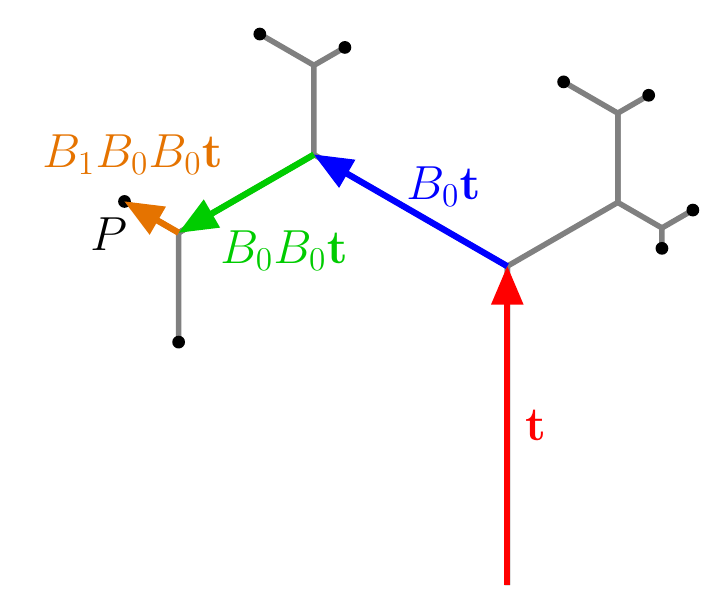
\begin{tikzpicture}[scale=1.8]
\def\nl{(-0.606218,1.35)}
\def\nr{(0.34641,1.2)}
\def\nll{(-1.03057,1.105)}
\def\nlr{(-0.606218,1.63)}
\def\nrl{(0.34641,1.48)}
\def\nrr{(0.484974,1.12)}
\def\nlll{(-1.03057,0.762)}
\def\nllr{(-1.20031,1.203)}
\def\nlrl{(-0.775959,1.728)}
\def\nlrr{(-0.509223,1.686)}
\def\nrll{(0.176669,1.578)}
\def\nrlr{(0.443405,1.536)}
\def\nrrl{(0.581969,1.176)}
\def\nrrr{(0.484974,1.056)}

\tikzstyle tree=[line width=0.07cm, gray]
\begin{scope}[xshift=3.75cm,yshift=0.35cm,scale=2.25]
\draw[tree] (0,0) -- (0,1) -- \nl -- \nll;
\draw[tree] \nlll -- \nll -- \nl -- \nlr -- \nlrr;
\draw[tree] \nll -- \nllr;
\draw[tree] \nlr -- \nlrl;
\draw[tree] (0,0) -- (0,1) -- \nr -- \nrl;
\draw[tree] \nrll -- \nrl -- \nr -- \nrr -- \nrrr;
\draw[tree] \nrl -- \nrlr;
\draw[tree] \nrr -- \nrrl;

\foreach \x in {\nlll,\nllr,\nlrl,\nlrr,\nrll,\nrlr,\nrrl,\nrrr} \fill[black] \x circle (0.02);
\LARGE
\draw[>=triangle 45,line width=0.08cm,->,red] (0,0) -- node[right] {\bf t} (0,1);

\draw[>=triangle 45,line width=0.08cm,->,blue] (0,1) --  \nl;

\draw[>=triangle 45,line width=0.08cm,->,green!80!black] \nl -- \nll;

\node[green!80!black] at (-0.7,1.05) {$B_0B_0\bf t$};

\node[blue] at (-0.2,1.25) {$B_0\bf t$};

\draw[>=triangle 45,line width=0.08cm,->,orange!90!black] \nll -- \nllr;

\node[orange!90!black] at (-1.175,1.35) {$B_1B_0B_0\bf t$};

\node at (-1.25,1.1) {$P$};
\end{scope}
\end{tikzpicture}
\end{center}

Now, we abstract a definition from this specific example.



Define $\Sigma=\{0,1,2,...,m-1\};$ $m$ will represent the number of branchings at each node of a tree. In the above example, $m=2.$

Define $\Sigma^n$ to be the set of all strings of length $n;$ elements of $\Sigma^n$ will represent sequences of instructions for traversing a binary tree. We denote the empty string by $\es,$ so that $\Sigma^0=\{\es\}.$  For $s\in\Sigma^n,$ we use $|s|=n$ to denote the length of $s.$ We say that $\Sigma^\omega$ is the set of all infinite strings with letters from $\Sigma,$ and put \begin{equation}
\Sigma^*=\Sigma^\omega\cup \bigcup_{n=0}^\infty \Sigma^n.
\end{equation}
Let $s_i$ denote the $i^{\rm th}$ letter in $s,$ and $s_{[i:j]}$ denote that substring of $s$ from the $i^{\rm th}$ to the $j^{\rm th}$ letter when $i\le j.$ When $i>j,$ we put $s_{[i:j]}=\es.$ Also, we write $\rev s$ for the string consisting of the letters of $s$ written in reverse order. This is fairly standard notation for strings used in many computer science applications.

Now let $\cal B$ be a finite set of $m$ affine transformations,  $\{B_0,\ldots B_{m-1}\}.$ These transformations describe how to create the branches in an $m$-ary tree. When all the transformations are invertible, we define ${\cal B}^{-1}$ to be the set of inverse transformations, $\{B_0^{-1},\ldots,B_{m-1}^{-1}\}.$

Now we look at (\ref{treedef}). We first need to define the individual terms of the sum.  To this end, we define, for a string $s$ of length $n,$
\begin{equation}
\eta_{\cal B}(s)=\prod_{i=1}^n B_{s_i} =B_{s_n}\ldots B_{s_1}.
\end{equation}

Note that $\eta_{\cal B}(\es)=I,$ and that the order of transformations in the product is important as the affine transformations may not commute. As an example, $\eta_{\cal B}(001)=B_1B_0B_0.$ Important here is that $\eta_{\cal B}$ defines a {\sl transformation,} not a {\sl vector.} This is because different trunk vectors may actually produce different trees even though the same $B_0$ and $B_1$ are used. Again, we strive for the greatest generality here.  

To add all the branches, we define, for $s\in\Sigma^n,$
\begin{equation}
\tau_{\cal B}(s)=\sum_{i=0}^{n} \eta_{\cal B}(s_{[1:i]}).
\end{equation}
For the above example, we have $s=001$ and
\begin{align*}
\tau_{\cal B}(001)&=\eta_{\cal B}(\Lambda)+\eta_{\cal B}(0)+\eta_{\cal B}(00)+\eta_{\cal B}(001)\\
&=I+B_0+B_0B_0+B_1B_0B_0.
\end{align*}

%For infinite strings, the analogous sum need not necessarily converge; when it does, we write
%\begin{equation}
%\tau_{\cal B}(s)=\sum_{i=0}^{\infty} \eta_{\cal B}(s_{[1:i]}).
%\end{equation}
%Note that this is a sum of transformations; we consider convergence with respect to the usual norm
%\begin{equation}
%\|M\|=\sup\{\|M{\bf v}\|\,|\,\|{\bf v}\|=1\}.
%\end{equation}
For $n\ge0,$ we define
\begin{equation}
{\cal C}^n_{\cal B}=\left\lbrace\tau_{\cal B}(s)\,|\,s\in\Sigma^n\right\rbrace.
\end{equation}
When a trunk (initial branch) {\bf t} of a tree is given, we call
\begin{equation}
{\cal C}_{\cal B}^n{\bf t}
\end{equation}
the {\bf canopy} of depth $n,$ and call elements of ${\cal C}_{\cal B}^n{\bf t}$ {\bf nodes} of depth $n.$ Defining a canopy in this way is important for us, since the number of nodes of depth $n$ often depends on the choice of trunk {\bf t.}

Of current interest is the sequence
\begin{equation}
|{\cal C}_{\cal B}^1{\bf t}|, |{\cal C}_{\cal B}^2{\bf t}|, |{\cal C}_{\cal B}^3{\bf t}|, |{\cal C}_{\cal B}^4{\bf t}|, |{\cal C}_{\cal B}^5{\bf t}|,\ldots,
\end{equation}
which we call the sequence of {\bf node numbers.} In other words, how many new nodes are created each time we iterate the binary tree algorithm? What we're finding is that an amazingly diverse range of sequences is possible, and moreover, that {\sl proving} the validity of any particular sequence is usually quite involved. 



\section{Definition of a Merkle tree}

Here, we discuss various useful notations and definitions for describing merkle trees.  


\begin{center}
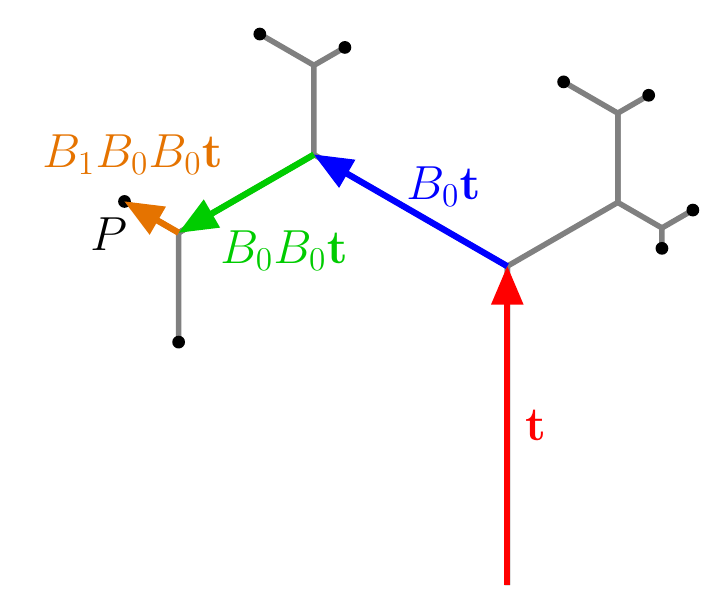
\begin{tikzpicture}[scale=1.8]
\def\nl{(-0.606218,1.35)}
\def\nr{(0.34641,1.2)}
\def\nll{(-1.03057,1.105)}
\def\nlr{(-0.606218,1.63)}
\def\nrl{(0.34641,1.48)}
\def\nrr{(0.484974,1.12)}
\def\nlll{(-1.03057,0.762)}
\def\nllr{(-1.20031,1.203)}
\def\nlrl{(-0.775959,1.728)}
\def\nlrr{(-0.509223,1.686)}
\def\nrll{(0.176669,1.578)}
\def\nrlr{(0.443405,1.536)}
\def\nrrl{(0.581969,1.176)}
\def\nrrr{(0.484974,1.056)}

\tikzstyle tree=[line width=0.07cm, gray]
\begin{scope}[xshift=3.75cm,yshift=0.35cm,scale=2.25]
\draw[tree] (0,0) -- (0,1) -- \nl -- \nll;
\draw[tree] \nlll -- \nll -- \nl -- \nlr -- \nlrr;
\draw[tree] \nll -- \nllr;
\draw[tree] \nlr -- \nlrl;
\draw[tree] (0,0) -- (0,1) -- \nr -- \nrl;
\draw[tree] \nrll -- \nrl -- \nr -- \nrr -- \nrrr;
\draw[tree] \nrl -- \nrlr;
\draw[tree] \nrr -- \nrrl;

\foreach \x in {\nlll,\nllr,\nlrl,\nlrr,\nrll,\nrlr,\nrrl,\nrrr} \fill[black] \x circle (0.02);
\LARGE
\draw[>=triangle 45,line width=0.08cm,->,red] (0,0) -- node[right] {\bf t} (0,1);

\draw[>=triangle 45,line width=0.08cm,->,blue] (0,1) --  \nl;

\draw[>=triangle 45,line width=0.08cm,->,green!80!black] \nl -- \nll;

\node[green!80!black] at (-0.7,1.05) {$B_0B_0\bf t$};

\node[blue] at (-0.2,1.25) {$B_0\bf t$};

\draw[>=triangle 45,line width=0.08cm,->,orange!90!black] \nll -- \nllr;

\node[orange!90!black] at (-1.175,1.35) {$B_1B_0B_0\bf t$};

\node at (-1.25,1.1) {$P$};
\end{scope}
\end{tikzpicture}
\end{center}

Now, we abstract a definition from this specific example.

Define $\Sigma=\{0,1,2,...,m-1\};$ $m$ will represent the number of branchings at each node of a tree. In the above example, $m=2.$








































\end{document}
